%!TEX root = ../CombinatoricsNotes.tex

\section{Tur\'an type problems} % (fold)
\label{sec:turian_type_problems}

The general problem we've been considering is to find $\max |\F|$ given that $\F\subset \P([n])$ has certain properties. For example, Sperner systems, and intersecting $r$-graphs. In these problems, we are forbidding certain sub set systems\sidenote{In a Sperner system, there is no 2 element sub system $\{A,B\}$ with $A\subset B$. In an intersecting $r$-graph, there is no two element sub system $\{A,B\}$ with $A\cap B= \emptyset$.}. Here, we will focus on $r$-graphs.  

We will say $\F$ and $\H$ are \defn{isomorphic} set systems if there exists a bijective map $\phi: \bigcup_{F\in \F} F \to \bigcup_{H\in \H}H$ such that $F\in \F$ if and only if $\phi(F)\in \H$.
Now, let forbidden subconfigurations $F_1,\dotsc,F_k$ be given $r$-graphs\sidenote{Recall: Set systems with elements which are in $[n]^{(r)}$.}. Define the \defn{Tur\'an number}
\[
\ex (n; F_1,\dotsc,F_k)
\]
to be the maximum $|\F|$ such that $\F$ does not contain a subgraph isomorphic to any of $F_1,F_2,\dotsc,F_k$.


\begin{remark}
We will increasingly refer to $F\in \F$ as edges.
\end{remark}

\begin{example}
If $M_2$ consists of two disjoint edges of size $r$, then \erdos-Ko-Rado says that $\ex(n;M_2) = {n-1\choose r-1}$ for $n\geq 2r$.\marginnote{Not having a subgraph isomorphic to $M_2$ means there must not be two disjoint subsets in $\F$, i.e., $\F$ is intersecting.}
\end{example}
Let
\[
\pi(n;F_1,\dotsc,F_k) := \frac{\ex(n;F_1,\dotsc,F_k)}{{n\choose r}}
\]
be the ratio of the largest valid size of $\F$ to the size of $[n]^{(r)}$.
We define the \defn{Tur\'an density} of $F_1,\dotsc,F_k$ to be
\[
\pi(F_1,\dotsc,F_k) := \lim_{n\to\infty} \pi(n; F_1,\dotsc,F_k) \in [0,1].
\]

\begin{example}
\[
\pi(M_2) = \lim_{n\to\infty} \frac{{n-1\choose r-1}}{{n\choose r}}=0,
\]
using \erdos-Ko-Rado. \marginnote{If you select two $r$-tuples of elments in an $n$ element set for very large $n$, you almost surely get disjoint tuples.}
\end{example}
\begin{theorem}[\cite{Katona_Nemetz_Simonovits}]
If $r\leq n_0\leq n$, then
\[
\pi(n_0; F_1,\dotsc,F_k) \geq \pi(n; F_1,\dotsc,F_k).
\]\label{thm:pi_decreasing}
\end{theorem}
\begin{remark}
Then $\pi(n;F_1,\dotsc,F_k)$ decreases for $n\geq r$ and is bounded below by zero,  so $\pi(F_1,\dotsc,F_k)$ exists.
\end{remark}
\begin{proof}	
Let $\F\subset[n]^{(r)}$ be such that $|\F| = \ex(n; F_1,\dotsc,F_k)$ and $\F$ contains no subgraphs isomorphic to any of $F_1,\dotsc, F_k$. Let $H_1,H_2,\dotsc,H_N$ be the restrictions\sidenote{Note that for $X\subset [n]$, we define the restriction of $\F$ as $\F\restriction X := \{A\in \F: A\subset X\}$.} of $\F$ to all possible $n_0$ element subsets of $[n]$, where $N = {n\choose n_0}$.
 It suffices to show that
% \begin{align}	\label{eq:pi_avg}
\[
\pi(n; F_1,\dotsc,F_k) = \frac{|\F|}{{n\choose r}} \leq \frac{1}{{n\choose n_0}} \sum_{i=1}^N \frac{|H_i|}{{n_0\choose r}}
\]
% \end{align}
since $\frac{|H_i|}{{n_0\choose r}} \leq \pi(n_0; F_1,\dotsc,F_k)$. \marginnote{This estimate is the only actual inequality in the proof.}

We are left to estimate $\sum_{i=1}^N|H_i|$.
Given an edge in $F\in\F$, how many $H_i$'s does it appear in? Each $H_i$ whose base set\sidenote{Meaning the $n_0$-element set $X$ such that $H_i = \F\restriction X$.} includes $F$, so we need to choose $n_0-r$ more elements for the base set from the $n-r$ remaining possible elements, i.e.  ${n-r \choose n_0-r}$.
Then,
\[
\frac{1}{{n\choose n_0}}\sum_{i=1}^N \frac{|H_i|}{{n_0\choose r}} = |\F| \frac{{n-r\choose n_0 -r}}{{n\choose n_0}{n_0\choose r}}\quad \boxed{=}\quad \frac{|\F|}{{n\choose r}}.
\]
To show the boxed equality and finish the proof, we need
\begin{equation}	\label{eq:binomial_identity_boxes}
{n\choose r}{n-r \choose n_0 -r} = {n\choose n_0}{n_0 \choose r}.
\end{equation}

\lect{2}{3}
% \marginnote[0\baselineskip]{Lecture 9: Wednesday, February 3, 2016}
This is an identity which we can combinatorially reason as follows. The RHS means we first choose $n_0$ elements out of $n$, then choose $r$ out of those $n_0$. The LHS means we choose $r$ elements from $n$ then $n_0-r$ elements from the remaining $n-r$. This is depicted in \cref{fig:binomial_identity_boxes}.

\begin{marginfigure}[0\baselineskip]
\begin{center}
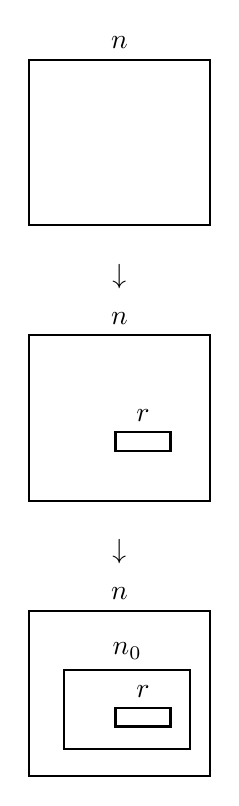
\begin{tikzpicture}

\begin{scope}
\node (rect) at (0,0)[draw,thick,minimum width=2.3cm, minimum height = 2.1cm, label=above:$n$]{};
% \node  at(.1,-.2)[draw,thick,minimum width=1.6cm, minimum height = 1cm, label=above:$n_0$]{};
% \node  at(.3,-.3)[draw,thick,minimum width=.7cm, minimum height = .2cm, label=above:$r$]{};
\end{scope}

\node[yshift=-1.7cm] at (0,0) {$\downarrow$};

\begin{scope}[yshift=-3.5cm]
\node (rect) at (0,0)[draw,thick,minimum width=2.3cm, minimum height = 2.1cm, label=above:$n$]{};
% \node  at(.1,-.2)[draw,thick,minimum width=1.6cm, minimum height = 1cm, label=above:$n_0$]{};
\node  at(.3,-.3)[draw,thick,minimum width=.7cm, minimum height = .2cm, label=above:$r$]{};
\end{scope}
\node[yshift=-5.2cm] at (0,0) {$\downarrow$};

\begin{scope}[yshift=-7cm]
\node (rect) at (0,0)[draw,thick,minimum width=2.3cm, minimum height = 2.1cm, label=above:$n$]{};
\node  at(.1,-.2)[draw,thick,minimum width=1.6cm, minimum height = 1cm, label=above:$n_0$]{};
\node  at(.3,-.3)[draw,thick,minimum width=.7cm, minimum height = .2cm, label=above:$r$]{};
\end{scope}
\end{tikzpicture}\hfill
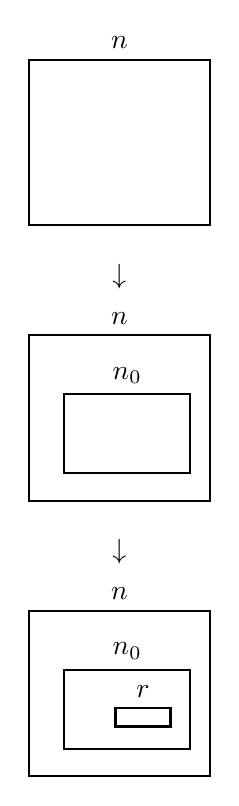
\begin{tikzpicture}
\begin{scope}
\node (rect) at (0,0)[draw,thick,minimum width=2.3cm, minimum height = 2.1cm, label=above:$n$]{};
% \node  at(.1,-.2)[draw,thick,minimum width=1.6cm, minimum height = 1cm, label=above:$n_0$]{};
% \node  at(.3,-.3)[draw,thick,minimum width=.7cm, minimum height = .2cm, label=above:$r$]{};
\end{scope}

\node[yshift=-1.7cm] at (0,0) {$\downarrow$};

\begin{scope}[yshift=-3.5cm]
\node (rect) at (0,0)[draw,thick,minimum width=2.3cm, minimum height = 2.1cm, label=above:$n$]{};
\node  at(.1,-.2)[draw,thick,minimum width=1.6cm, minimum height = 1cm, label=above:$n_0$]{};
% \node  at(.3,-.3)[draw,thick,minimum width=.7cm, minimum height = .2cm, label=above:$r$]{};
\end{scope}
\node[yshift=-5.2cm] at (0,0) {$\downarrow$};

\begin{scope}[yshift=-7cm]
\node (rect) at (0,0)[draw,thick,minimum width=2.3cm, minimum height = 2.1cm, label=above:$n$]{};
\node  at(.1,-.2)[draw,thick,minimum width=1.6cm, minimum height = 1cm, label=above:$n_0$]{};
\node  at(.3,-.3)[draw,thick,minimum width=.7cm, minimum height = .2cm, label=above:$r$]{};
\end{scope}
\end{tikzpicture}
\end{center}
\caption{(above) \emph{Left:} an illustration of the LHS of \cref{eq:binomial_identity_boxes} and \emph{right:} the RHS of \cref{eq:binomial_identity_boxes}. } \label{fig:binomial_identity_boxes}
\end{marginfigure}
\end{proof}

Let $H$ be a graph ($2$-graph). Then $\ex(n,H)=\max |\edges (G)|$, where the maximum is taken over graphs $G$ with $|V(G)| = n$ such that $H$ is not a subgraph of $G$.

We may consider
\[	
\pi(n;H) := \frac{\ex(n,H)}{{n\choose 2}}, \qquad \pi(H):= \lim_{n\to \infty}\pi(n,H).
\]
By \cref{thm:pi_decreasing}, $\pi(n,H)$ decreases for $n\geq 2$ (and fixed $H$), so $\pi(H)$ exists. Let $K_n$ be the complete graph on $n$ verticies: $K_n = [n]^{(2)}$. Since $K_2$ is just a single edge, $\ex(n; K_2)=0$.

Consider
$P_3 =$\scalebox{1}{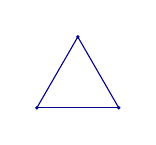
\begin{tikzpicture}[color=DarkBlue]
\def\n{3}
\def\radius{.6}
\def\rotation{-30}

\def\deg{360/\n}
\pgfmathsetmacro\nminusone{\n-1}

\foreach \x in {1,...,\n}
{
	\pgfmathsetmacro\myangle{\x*\deg+\rotation};
	\filldraw (\myangle:\radius cm) circle (0.4pt) node(a\x){};
}


\foreach \y in {1,...,\n}
{

	\foreach \z in {1,...,\y}
	{
		\ifthenelse{\z < \nminusone}
		{
		\pgfmathsetmacro\myangley{\y*\deg+\rotation}
		\pgfmathsetmacro\myanglez{\z*\deg+\rotation}
		\draw (\myangley:\radius cm) -- (\myanglez:\radius cm);
		}{}

	}
}
\end{tikzpicture}}. Then $\ex(n,P_3) = \floor{n/2}$, and $\pi(P_3)=0$.

Consider $K_3 =$\scalebox{1}{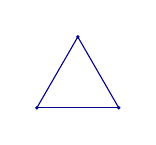
\begin{tikzpicture}[color=DarkBlue]
\def\n{3}
\def\radius{.6}
\def\rotation{-30}

\def\deg{360/\n}
\pgfmathsetmacro\nminusone{\n-1}

\foreach \x in {1,...,\n}
{
	\pgfmathsetmacro\myangle{\x*\deg+\rotation};
	\filldraw (\myangle:\radius cm) circle (0.4pt) node(a\x){};
}


\foreach \y in {1,...,\n}
{

	\foreach \z in {1,...,\y}
	{
		\ifthenelse{\z < \n}
		{
		\pgfmathsetmacro\myangley{\y*\deg+\rotation}
		\pgfmathsetmacro\myanglez{\z*\deg+\rotation}
		\draw (\myangley:\radius cm) -- (\myanglez:\radius cm);
		}{}

	}
}
\end{tikzpicture}}.
Let us bound $\pi(K_3)$. Consider $n$ even, and the complete bipartite graph on $n$ verticies, shown in \cref{fig:bipartite}.

\begin{figure}
\begin{center}
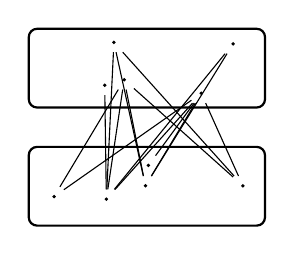
\begin{tikzpicture}[color=black]

\node (rect) at (0,0)[draw,thick,minimum width=3cm, minimum height = 1cm, rounded corners=3pt]{};

\node (rect2) at (0,1.5)[draw,thick,minimum width=3cm, minimum height = 1cm, rounded corners=3pt]{};

\pgfmathsetseed{3}
% \def\z{rand}
\foreach \x in {1,...,5}
{
\filldraw (rand*1.4,rand*.4) circle (0.4pt) node(a\x){};
\filldraw (rand*1.4,1.5+rand*.4) circle (0.4pt) node(b\x){};

}

\foreach \x in {1,...,5}
{
% \ifthenelse{\x > 1}{\draw[dashed] (a\x) -- (u)}{};
\foreach \y in {1,...,\x}
{
\draw (a\x) -- (b\y);
}
}

\end{tikzpicture}
\end{center}
\caption[][1cm]{(left) The complete bipartite graph on $n$ verticies. We divide the graph into independent sets of size $n/2$, then connect each vertex in the upper set to each vertex in the lower set. This produces $(n/2)^2$ edges and no triangles. \label{fig:bipartite}}
\end{figure}


 Then $\pi(n,K_3) \geq \frac{n^2/4}{{n\choose 2}} \to \frac{1}{2}$. On the other hand, $P_3$ achieves 
 \[	
 \pi(3,K_3) = \frac{\ex(3,K_3)}{3} = \frac{2}{3},
 \]
 so by \cref{thm:pi_decreasing},  $\pi(K_3)\leq \frac{2}{3}$.
Thus, we have
\[	
\frac{1}{2}\leq \pi(K_3)\leq \frac{2}{3}.
\]

How do we make a graph with many edges that does not contain any complete subgraphs on $t$ verticies?

We look at $t$ groups of size $\frac{n}{t}$. Then join two verticies if they lie in different groups, but not join them if they lie in the same group.


\begin{figure}
\begin{center}
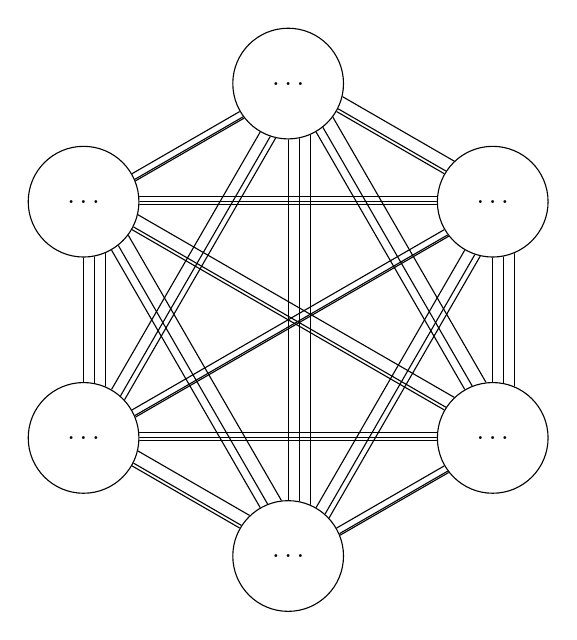
\begin{tikzpicture}
\begin{scope}
% \node[left] at (0,0) {$\circlearrowleft$};


\foreach \y in {1,...,6}
{
\foreach \z in {1,...,\y}
{
\pgfmathsetmacro\myangley{-1*\y*60+90}
\pgfmathsetmacro\myanglez{-1*\z*60+90}
\draw (\myangley:3cm) -- (\myanglez:3cm);
\draw[xshift=4pt,yshift=-1pt] (\myangley:3cm) -- (\myanglez:3cm);
\draw[xshift=8pt,yshift=2pt] (\myangley:3cm) -- (\myanglez:3cm);
}
}
 % do a few by hand
 \pgfmathsetmacro\myangley{-1*3*60+90}
 \pgfmathsetmacro\myanglez{-1*5*60+90}
% \draw (\myangley:3cm) -- (\myanglez:2.9cm);



\foreach \x in {1,...,6}
{
 \pgfmathsetmacro\myangle{-1*\x*60+90}

\ifthenelse{\x > 1}{
\filldraw[white] (\myangle:3cm) circle (20pt);
\draw[black] (\myangle:3cm) circle (20pt) node{$\frac{n}{t}$
};
}{
\filldraw[white] (\myangle:3cm) circle (10pt);
\draw (\myangle:3cm) node[auto]{$\ldots$};
};

}


%  \pgfmathsetmacro\myangle{-1*60+90}
% \draw (\myangle:3cm) node[auto]{$\ldots$};

\end{scope}
\end{tikzpicture}
\end{center}
\caption{The Tur\'an graph on $n$ verticies, in the case that $n$ is divisible by $t$. We partition the graph into $t$ independent subsets of size $\frac{n}{t}$. Then we connect each vertex in each independent subset $A$ to all the verticies in $V(G)\setminus A$.  \label{fig:turan_graph}}
\end{figure}
% Connect each circle to every other circle, several times.


The \defn{Tur\'an graph} $T_t(n)=T$ is a graph with $|V(T)|=n$ such that $V(T)$ is  partitioned into $A_1,\dotsc,A_{t}$ and $v\in A_i$ is adjacent to $u\in A_j$ iff $i\neq j$, and the sizes obey $||A_i| - |A_j|| \leq 1$ for all $i,j$.

Then
\[
\pi(K_t) \geq \lim_{n\to\infty} \frac{|\edges (T_{t-1}(n))|}{{n\choose 2}} = \lim_{n\to\infty} \frac{{n\choose 2} - (t-1){\frac{n}{t-1} \choose 2}}{{n\choose 2}}= 1 - \frac{1}{t-1} = \frac{t-2}{t-1}
\]

\begin{theorem}[\cite{turan1941extremal}] \label{thm:turan}
For every $t\geq 2$, $\pi(K_t) = \frac{t-2}{t-1}$. Moreover,
\[
\ex(n,K_t)\leq \frac{t-2}{t-1} \frac{n^2}{2}.
\]
\end{theorem}
\begin{proof}[Proof by induction on $n$.] 
Note that when $n$ is divisible by $t-1$,
\[
\ex(n,K_t)\geq |\edges (T_{t-1}(n))| = \frac{t-2}{t-1}\frac{n^2}{2}
\]
and equality is acheived.
Base case: for $n < t-1$, then the maximal number of edges (without restriction) is ${n\choose 2}  = \frac{n-1}{n}\frac{n^2}{2}\leq \frac{t-2}{t-1}\frac{n^2}{2}$.

Induction step. Let $n\geq t-1$. We may assume that $K_{t-1}$ is a subgraph of our graph $G$ (where $G$ is a graph on verticies with no $K_t$ subgraph and $|\mathcal{G}| = \ex(n,K_t)$.

Let $U=\{v_1,v_2,\dotsc,v_{t-1}\}$ be the set of verticies of this $K_{t-1}$ subgraph. Then
\[	
 |\edges (G) | = \frac{(t-1)(t-2)}{2} + | \edges (U,V(G)\setminus U)| + |\edges (G\setminus U)|.
 \]
 This is the number of edges within $U$, plus the number of edges with exactly one end in $U$, plus the number of edges not connected to $U$, respectively. See \cref{fig:U_VG-U} for a depiction of this partition.

 % \missingfigure{partition of $G$ into $U$ and $V(G)\setminus U$. $U$ is a complete graph. Put a point $u$ in the latter.}
\begin{marginfigure}
\begin{center}
\begin{tikzpicture}
\node (rect) at (0,0)[draw,thick,minimum width=1cm, minimum height = 2cm, rounded corners=3pt,label=above:$U\cong K_{t-1}$]{};

\node (rect2) at (2,0)[draw,thick,minimum width=1cm, minimum height = 2cm, rounded corners=3pt,label=above:$V(G)\setminus U$]{};

\pgfmathsetseed{3}
% \def\z{rand}
\foreach \x in {1,...,5}
{
\filldraw[black] (rand*.5,rand*1) circle (0.4pt) node(a\x){};
}
% \draw (a1) -- (a2);

\filldraw[black] (2,.5) circle (0.4pt) node[right](u){$u$};



\foreach \x in {1,...,5}
{
\ifthenelse{\x > 1}{\draw[dashed] (a\x) -- (u)}{};
\foreach \y in {1,...,\x}
{
\draw (a\x) -- (a\y);
}
}

% \filldraw at (rect2)[draw, fill=black,circle(.4pt),above,label=above:$u$]{};

\end{tikzpicture}
\end{center}
\caption{ Illustation of the partition of $G$ into $V(G)\setminus U \ni u$ and $U$. If $u$ were adjacent to more than $t-2$ notes in $U$, then $U\cup \{u\} \cong K_t$. \label{fig:U_VG-U}}
\end{marginfigure}



 For every $u\in V(G)\setminus U$, the vertex $u$ is adjacent to $\leq t-2$ verticies in $U$ (otherwise $U\cup\{u\}\cong K_t$). So
 \[
 \edges (U,V(G)-U)| \leq (t-2) |V(G)-U| = (t-2)(n-t-1).
 \]

 Moreover,
 \[
 |\edges (G\setminus U)|  \leq \frac{t-2}{t-1}\frac{(n-t+1)^2}{2},
 \]
 by the induction hypothesis. Putting it all together,
 \begin{align*}
 |\edges (G)| &\leq \frac{(t-1)(t-2)}{2} + (t-2)(n-t+1) + \frac{t-2}{t-1}\frac{(n-t+1)^2}{2}\\
 &= \frac{t-2}{2(t-1)} \left( (t-1)^2 + 2(t-1) (n-t+1) + (n-t+1)^2 \right)\\
 &= \frac{t-2}{2(t-1)} n^2.\qedhere
 \end{align*}
\end{proof}
\lect{2}{8}
% \marginnote{Lecture 10: Monday, February 8, 2016.}
We'll provide another proof of Tur\'an's theorem, but first let us introduce some notation. Let 
\[
d(G) = \frac{2|\edges (G)|}{n^2}
\]
be the \defn{density}[density of graph] of $G$; this is the probability that choosing two verticies uniformly at random (with repetition) from $V(G)$ gives an edge. The density $\lambda$ is called the \defn{Lagrangian} of $G$.

Suppose $V(G) = [n]$. Let 
\[
\lambda(G) := \max_{\substack{x_i\geq 0,\\ \sum_{i=1}^n x_i=1}} \sum_{(i,j) \in \edges (G)} x_i x_j.
\]
Then $2\lambda(G)$ is the maximum probability of selecting an edge by independently sampling two verticies taken over all probability distributions on the vertex set. In particular, $2\lambda(G) \geq d(G)$, for every $G$.

\begin{example}
\[
\lambda(K_2) = \max_{\substack{x_1,x_2\geq 0 \\ x_1+x_2=1}} x_1 x_2 =\max_{x_1\geq 0} x_1(1-x_1) = \frac{1}{4},
\]
achieved when $x_1=x_2=\frac{1}{2}$.

\[
\lambda(P_3) = \max_{\substack{x_1,x_2,x_3\geq 0\\ x_1+x_2+x_3}} x_1x_2 + x_2x_3 = \max_{\substack{x_1,x_2,x_3\geq 0\\ x_1+x_2+x_3}} x_2(x_1+x_3)
\]
is still a product of two things which sum to one. So we need $x_2=\frac{1}{2}$ and $x_1+x_3=\frac{1}{2}$. We could take $x_1=x_3=\frac{1}{4}$.
\end{example}

\begin{lemma}
$\lambda(K_t) = \frac{t-1}{2 t}$.
\end{lemma}
\begin{proof}	
The uniform distribution on $|V(K_t)|$ acheives $\frac{t-1}{2t}$, so it is enough to show
\[
\sum_{\substack{1\leq i<j \leq t,\\ x_i\geq 0,\\ \sum_{i=1}^n x_i=1.}} x_i x_j \leq \frac{t-1}{2t}.
\]
But
\[
\sum_{\substack{1\leq i<j \leq t,\\ x_i\geq 0,\\ \sum_{i=1}^n x_i=1.}} 2x_i x_j  = (x_1+x_2+\dotsm + x_t)^2 - \sum_{i=1}^t x_i^2 = 1- \sum_{i=1}^t x_i^2 \quad\boxed{\leq} \quad 1 - \frac{1}{t}
\]
where we need to show the boxed inequality.
Equivalently, we need $\sum_{i=1}^t x_i^2 \geq \frac{1}{t}$ for all $x_i$ as above. But this follows from Jensen's inequality (with the uniform distribution): if $f$ is convex, then
\[
\frac{\sum_{i=1}^n f(x_i)}{n} \geq f \left( \frac{x_1+\dotsm + x_n}{n}\right)
\]
for all $x_1,\dotsc,x_n$. 

Here, we take $f(x)=x^2$, to obtain
\[
\frac{\sum_{i=1}^n x_i^2}{t}\geq \left(\frac{x_1+\dotsm + x_t}{t}\right)^2 = \left( \frac{1}{t} \right)^2. \qedhere
\]
\end{proof}

\begin{theorem} \label{thm:lambda_G}
If $G$ has no $K_t$ subgraph, then $\lambda(G) \leq \lambda(K_{t-1}) = \frac{t-2}{2(t-1)}$.
\end{theorem}
\begin{proof}	
Let $p_G(\bar x) = \sum_{\{i,j\}\in \edges (G)} x_i x_j$. Then
\[
\lambda(G) = \max_{\substack{x_i\geq 0 \\ \sum_i x_i =1}} p_G(\bar x).
\]
Choose maximal $\bar x$ so that $p_G(\bar x) = \lambda(G)$, and $\#\{i: x_i \neq 0\}$ is minimal.
We may assume that in fact $x_i>0$ for all $i$, by throwing away verticies with zero weights.
\begin{claim}
$G$ is complete.
\end{claim}
\begin{remark}
This means the probability distribution was concentrated on a complete subgraph.
\end{remark}
\begin{subproof}[Proof of claim]
Suppose $G$ is not complete. Then there exists $i,j\in V(G)$ non-adjacent. We have
\begin{align*}	
p_G(\bar x) &= x_i \overbrace{\sum_{\substack{k: \\ \{k,i\} \in \mathcal{G}(G)}} x_k}^{C_i} + x_j \overbrace{ \sum_{\substack{k: \\ \{k,j\} \in \mathcal{G}(G)}} x_k}^{C_j} + \overbrace{\sum_{\substack{\{k,\ell\} \in \edges (G):\\ k,\ell \in V(G)\setminus \{i,j\} }} x_k x_\ell}^{b}.
\end{align*}
Assume wlog that $C_j\geq C_i$. Let $\bar x'$ be obtained by setting $x'_i=0$ and $x'+j = x_i + x_j$, and the other $x'_k = x_k$ (for $k\neq j$ and $k\neq i$). Then $p_G(\bar x') = (x_i+x_j) C_j + b \geq x_i C_i + x_j C_j + b = p_G(\bar x)$.

This is a contradiction: $\bar x'$ has more zero values than $\bar x$, but still acheives $\lambda(G)$. But we choose $\bar x$ to have the minimal number of non-zero values.
 % But since $\bar x$ is maximal, we must have $C_i = C_j$.
\end{subproof}
Then $G$ is complete, and so must be of size $t-1$.
\end{proof}

\begin{remark}
 \Cref{thm:lambda_G} proves \cref{thm:turan}.
\end{remark}
\begin{proof}	
\[
\frac{|\edges (G)|}{n^2}=p_G(\frac{1}{n}, \dotsc, \frac{1}{n}) \leq\lambda(G) \leq \frac{t-2}{2(t-1)}.\qedhere
\]
\end{proof}
\lect{2}{10}
% \marginnote{Lecture 11: Wednesday, February 10, 2016.}

Let $K_{1,t}$ be the graph \scalebox{.5}{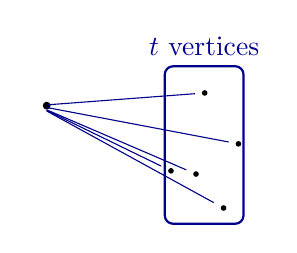
\begin{tikzpicture}[color=DarkBlue]
\node (rect) at (0,0)[draw,thick,minimum width=1cm, minimum height = 2cm, rounded corners=3pt,label=above:{$t$ vertices}]{};

% \node (rect2) at (2,0)[draw,thick,minimum width=1cm, minimum height = 2cm, rounded corners=3pt,label=above:$V(G)\setminus U$]{};

\pgfmathsetseed{3}
% \def\z{rand}
\foreach \x in {1,...,5}
{
\filldraw[black] (rand*.5,rand*1) circle (0.8pt) node(a\x){};
}
% \draw (a1) -- (a2);

\filldraw[black] (-2,.5) circle (1.2pt) node[left](u){};



\foreach \x in {1,...,5}
{
\draw (a\x) -- (u);
}

% \filldraw at (rect2)[draw, fill=black,circle(.4pt),above,label=above:$u$]{};

\end{tikzpicture}}.
Then $\pi(K_{1,t})= 0$, as follows:
We may bound
\[	
\ex(n,K_{1,t}) \leq \frac{(t-1)n}{2}
\]
because every vertex has degree $\leq t-1$ if there is no $K_{t,1}$ subgraph.



Let $K_{2,2}$ be the graph 
\scalebox{.7}{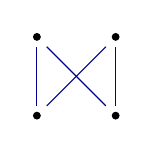
\begin{tikzpicture}[color=DarkBlue]
\filldraw[black] (0,0) circle (1.2pt) node(a1){};

\filldraw[black] (0,1) circle (1.2pt) node(a2){};


\filldraw[black] (1,0) circle (1.2pt) node(a3){};
\filldraw[black] (1,1) circle (1.2pt) node(a4){};
\draw (a3) -- (a4);

\draw (a1) -- (a2);

\draw (a2) -- (a3);

\draw (a1) -- (a4);



% \foreach \x in {1,...,4}
% {
% \foreach \y in {1,...,2}
% {
% \draw (a\x) -- (a\y);
% }
% }

\end{tikzpicture}}.
If $G$ has no $K_{2,t}$ then it has $\leq (t-1){n\choose 2}$ paths $P_3$ as subgraphs, but if $G$ has $\epsilon {n\choose 2}$ edges, we ``expect'' $\geq \epsilon^2 {n\choose 3}$ paths $P_3$, so if $\epsilon>0$ for large $n$, we get a contradiction.
Thus, $\pi(K_{2,t})=0$.



\begin{theorem}
$\pi(K_{t,t})=0$ for every $t>1$.
\end{theorem}
\begin{remark}
This implies $\pi(H)=0$ for every bipartite graph $H$.
\end{remark}
\begin{proof}	
We need to show that for every $\epsilon>0$ there exists $n_0$ such that if $G$ has no $K_{t,t}$ subgraph, and $n\geq n_0$ verticies, then $|\edges (G)|\leq \epsilon{n\choose 2}$.


Suppose that $|\edges (G)|\geq \epsilon {n\choose 2}$.



\begin{figure}
\begin{center}
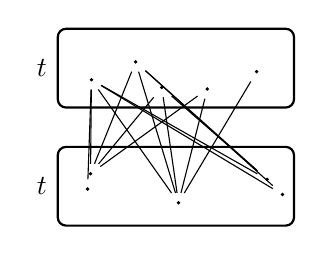
\begin{tikzpicture}[color=black]

\node (rect) at (0,0)[draw,thick,minimum width=3cm, minimum height = 1cm, rounded corners=3pt, label=left:$t$]{};

\node (rect2) at (0,1.5)[draw,thick,minimum width=3cm, minimum height = 1cm, rounded corners=3pt,label=left:$t$]{};

\pgfmathsetseed{4}
% \def\z{rand}
\foreach \x in {1,...,5}
{
\filldraw (rand*1.4,rand*.3) circle (0.4pt) node(a\x){};
\filldraw (rand*1.4,1.5+rand*.3) circle (0.4pt) node(b\x){};

}

\foreach \x in {1,...,5}
{
% \ifthenelse{\x > 1}{\draw[dashed] (a\x) -- (u)}{};
\foreach \y in {1,...,\x}
{
\draw (a\x) -- (b\y);
}
}

\end{tikzpicture}
\end{center}
\caption[][0cm]{Left. The bipartite graph on $n$ verticies. We divide the graph into independent sets of size $n/2$, then connect each vertex in the upper set to each vertex in the lower set. This produces $(n/2)^2$ edges and no triangles. \label{fig:bipartite2}}
\end{figure}

Set
\[
f(G) = \sum_{\{v_1,v_2,\dotsc,v_t\}\subset V(G)^{(t)}} | N(v_1)\cap N(v_2)\dotsm \cap N(v_t)| \leq (t-1){n\choose t}
\]
where $N(v)$ is the set of neighbors of $v$ in $G$: that is, $N(v) = \{u\in V(G): \{u,v\} \in \edges (G) \}$.



We are counting subgraphs of the form
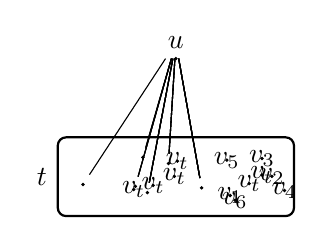
\begin{tikzpicture}[color=black]

\node (rect) at (0,0)[draw,thick,minimum width=3cm, minimum height = 1cm, rounded corners=3pt, label=left:$t$]{};
\filldraw (0,1.5) circle (0.4pt) node[above](u){$u$};

% \node (rect2) at (0,1.5)[draw,thick,minimum width=3cm, minimum height = 1cm, rounded corners=3pt,label=left:$t$]{};

\pgfmathsetseed{3}
% \def\z{rand}
\foreach \x in {1,...,6}
{
\ifthenelse{\x>5}{
\filldraw (rand*1.4,rand*.3) circle (0.4pt) node(a\x){$v_t$};
	
}{
\ifthenelse{\x<3}{

\filldraw (rand*1.4,rand*.3) circle (0.4pt) node(a\x){$v_\x$}; }{
	\filldraw (rand*1.4,rand*.3) circle (0.4pt) node(a\x){};
};
	
};
% \filldraw (rand*1.4,1.5+rand*.3) circle (0.4pt) node(b\x){};

}

\foreach \x in {1,...,6}
{
% \ifthenelse{\x > 1}{\draw[dashed] (a\x) -- (u)}{};
\foreach \y in {1,...,\x}
{
\draw (a\x) -- (u);
}
}

\end{tikzpicture}.

First, note
\[
{m\choose t} \geq \frac{m^t}{t!} - cm^{t-1}
\]
for some constant $c$ depending on $t$ only.

Then,
\begin{align*}	
f(G) &= \sum_{u\in V(G)} {\deg (u) \choose t} \geq \sum_{u\in V(G)} \left( \frac{\deg^t(u)}{t!}- c \deg^{t-1}(u) \right)\\
\intertext{where we've used Jensen's for $t$th powers. Then,}
&\geq \frac{n}{t!} \left( \sum_{u\in V(G)} \frac{\deg(u)}{n} \right)^t - cn^t\\
&\geq \frac{n}{t!} \left( \frac{2 \epsilon {n\choose 2}}{n} \right)^t - cn^t\\
\intertext{Using $2 \epsilon {n\choose 2} \geq \frac{\epsilon}{2}n^2$}
&\geq \frac{n}{t!}\left( \frac{\epsilon}{2}n \right)^t - cn^t\\
& \boxed{>} (t-1) {n \choose t}
\end{align*}
where the boxed inquality yields a contradiction, and holds for large enough $t$.
\end{proof}


If $H$ is not bipartite, is it possible $\pi(H)=0$? No, there exist large ``dense'' graphs with no $H$ subgraph.
For every non-bipartite graph, the Tur\'an density is at least 1/2, for the same reason as $K_3$: it cannot be embedded in a large complete bipartite graph, so these graphs\sidenote[][-2cm]{which have density 1/2} witness this.


Let us consider graphs which are not subgaphs of the Tur\'an graph $T_{3}(n)$ (depicted in \cref{fig:T3}): 
If $H$ is not a subgraph of $T_3(n)$ for any $n$, then $\pi(H)\geq \frac{2}{3}$. Let us generalize.
\begin{marginfigure}[-2cm]
\begin{center}
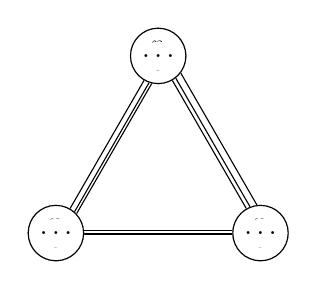
\begin{tikzpicture}[scale=.5]
\begin{scope}
% \node[left] at (0,0) {$\circlearrowleft$};


\foreach \y in {1,...,3}
{
\foreach \z in {1,...,\y}
{
\pgfmathsetmacro\myangley{-1*\y*120+90}
\pgfmathsetmacro\myanglez{-1*\z*120+90}
\draw (\myangley:3cm) -- (\myanglez:3cm);
\draw[xshift=4pt,yshift=-1pt] (\myangley:3cm) -- (\myanglez:3cm);
\draw[xshift=8pt,yshift=2pt] (\myangley:3cm) -- (\myanglez:3cm);
}
}
 % do a few by hand
 \pgfmathsetmacro\myangley{-1*3*120+90}
 \pgfmathsetmacro\myanglez{-1*5*120+90}
% \draw (\myangley:3cm) -- (\myanglez:2.9cm);



\foreach \x in {1,...,6}
{
 \pgfmathsetmacro\myangle{-1*\x*120+90}

\ifthenelse{\x > 1}{
\filldraw[white] (\myangle:3cm) circle (20pt);
\draw[black] (\myangle:3cm) circle (20pt) node{$\frac{n}{3}$
};
}{
\filldraw[white] (\myangle:3cm) circle (10pt);
\draw (\myangle:3cm) node[auto]{$\ldots$};
};

}


%  \pgfmathsetmacro\myangle{-1*60+90}
% \draw (\myangle:3cm) node[auto]{$\ldots$};

\end{scope}
\end{tikzpicture}
\end{center}
\caption{The Tur\'an graph $T_3(n)$.} \label{fig:T3}
\end{marginfigure}


% \begin{definition}%[$k$-coloring, $\chi(G)$]
 We say $c\!\!: V(G) \to [k]$ is a \defn{$k$-coloring} if $c(u)\neq c(v)$ for every $\{u,v\}\in \edges (G)$.

We write $\chi(G)$ for the minimum $k$ such that $G$ admits a $k$-coloring. With this definition in hand, we may formulate the following result.
% \end{definition}
\begin{lemma} \label{lem:min_Tur\'an_density_2graphs}
If $H$ contains an edge,
\[
\pi(H)\geq \frac{\chi(H)-2}{\chi(H)-1}.
\]
\end{lemma}

\begin{proof}	
Let $k = \chi(H)-1$. As $H$ is not $k$-colorable, $H$ is not a subgraph of any Tur\'an graph $T_k(n)$ and so $\pi(H)\geq \lim_{n\to\infty} \frac{|\edges (T_k(n))|}{{n\choose 2}} = \frac{k-1}{k}$.
\end{proof}

\begin{lemma} \label{lem:subgraph_with_min_vertex_degree}
For every $r$, $n_0$, and $\epsilon$, there exists $N$ such that if $G$ is an $r$-graph with $|V(G)| = n\geq N$ and $|\edges (G)|\geq d {n\choose r}$, then $G$ contains a subgraph (sub $r$-graph) $G'$ such that
\[
|V(G')| =n' \geq n_0
\]
and every vertex $v\in V(G')$ belongs to at least $(d - \epsilon) {n' \choose r-1}$ edges.
\end{lemma}
\marginnote{So we can  restrict to a (large) subgraph to obtain a minimal bound on vertex degree, at the cost of $\epsilon$ density. }
\begin{proof}	
Suppose not. Then there exists a vertex $v_1\in V(G)$ such that $v_1$ belongs to at most $(d - \epsilon) {n \choose r-1}$ edges. Delete this vertex to obtain a graph $G_1$ which in turn has a vertex $v_2$ in at most $(d- \epsilon){n-1 \choose r-1}$ edges. Delete this vertex to obtain $G_2$, and continue in the same manner.

We eventually arrive at a graph $G_{n-n_0}$ on $n_0$ verticies. Then
\begin{fullwidth}
\begin{align*}	
d {n \choose r} &\leq |G| \\
&\leq (d -\epsilon){n\choose r-1} + (d- \epsilon) {n-1 \choose r-1} + \dotsm + (d- \epsilon){n_0+1 \choose r-1} + \underbrace{|G_{n-n-0}|}_{\leq {n_0\choose r}}.
\end{align*}
It remains to show that for $n$ large enough (in terms of $n_0,r,\epsilon$)
\[
d {n \choose r} > (d- \epsilon) \left[{n\choose r-1} +  {n-1 \choose r-1} + \dotsm + {n_0+1 \choose r-1}  \right] + {n_0 \choose r}.
\]
But, repeating the Pascal's triangle inequality,
\[
{n\choose r} = {n-1 \choose r-1} + {n-2\choose r-1} + {n-3 \choose r-1} + \dotsm + {r-1 \choose r-1}.
\]
So,
\[
d {n\choose r} = (d - \epsilon) \left( {n-1 \choose r-1} + {n-2\choose r-1} + {n-3 \choose r-1} + \dotsm + {r-1 \choose r-1} \right) + \epsilon {n\choose r}.
\]
\end{fullwidth}

This eliminates most terms; we are left with
\[
\epsilon {n\choose r} \overset{?}{>} (d- \epsilon) {n\choose r-1} + {n_0 \choose r}.
\]
But the polynomial in $n$ on the left has degree $r$, and on the right, degree $r-1$, so for $n\geq N$ with $N$ large enough, we have strict inequality.

\end{proof}

\begin{theorem}[\cite{erdos-stone}]
\[
\pi(H) = \frac{\chi(H)-2}{\chi(H)-1}
\]
for every $2$-graph $H$ with $\chi(H)\geq 2$\marginnote{I.e. $H$ contains an edge.}.
\end{theorem}
\begin{proof}	
\Cref{lem:min_Tur\'an_density_2graphs} gives the lower bound. Now, consider $K_{\underbrace{t,\dotsc,t}_{k \text{ times}}}$ the complete $k$-partite graph with parts of size $t$, as depicted in \cref{fig:Ktttt}.
\begin{figure}
\begin{center}
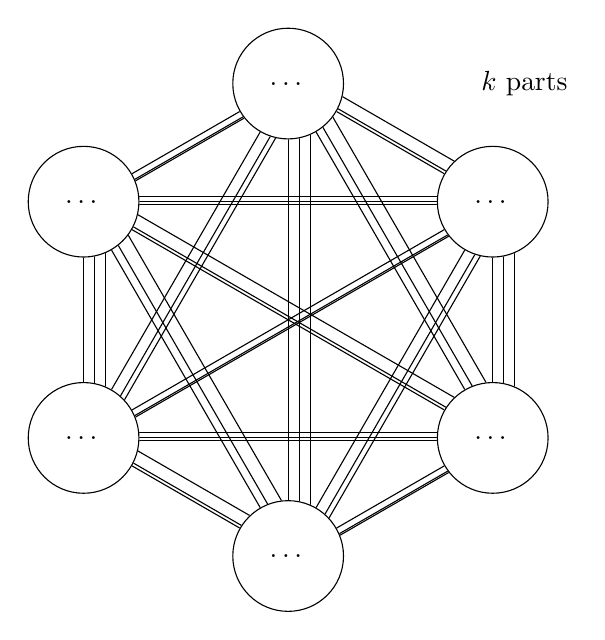
\begin{tikzpicture}
\begin{scope}
% \node[left] at (0,0) {$\circlearrowleft$};


\foreach \y in {1,...,6}
{
\foreach \z in {1,...,\y}
{
\pgfmathsetmacro\myangley{-1*\y*60+90}
\pgfmathsetmacro\myanglez{-1*\z*60+90}
\draw (\myangley:3cm) -- (\myanglez:3cm);
\draw[xshift=4pt,yshift=-1pt] (\myangley:3cm) -- (\myanglez:3cm);
\draw[xshift=8pt,yshift=2pt] (\myangley:3cm) -- (\myanglez:3cm);
}
}
 % do a few by hand
 \pgfmathsetmacro\myangley{-1*3*60+90}
 \pgfmathsetmacro\myanglez{-1*5*60+90}
% \draw (\myangley:3cm) -- (\myanglez:2.9cm);



\foreach \x in {1,...,6}
{
 \pgfmathsetmacro\myangle{-1*\x*60+90}

\ifthenelse{\x > 1}{
\filldraw[white] (\myangle:3cm) circle (20pt);
\draw[black] (\myangle:3cm) circle (20pt) node{$t$
};
}{
\filldraw[white] (\myangle:3cm) circle (10pt);
\draw (\myangle:3cm) node[auto]{\ldots};
};

}
\draw (3,3) node[auto]{$k$ parts};


%  \pgfmathsetmacro\myangle{-1*60+90}
% \draw (\myangle:3cm) node[auto]{$\ldots$};

\end{scope}
\end{tikzpicture}
\end{center}
\caption{An illustration of $K_{tt\dotsm  t}$, where there are $k$ $t$'s in the subscript. This means we have $k$ independent sets of size $t$, and each vertex of each independent set is connected to all the vertices in all the other sets.  \label{fig:Ktttt}}
\end{figure}


For every $t$,
\[	
\pi(K_{t,\dotsc,t}) \leq \frac{k-2}{k-1}
\]
by induction on $k$. Suppose for some $k$, and some $t$,
\[	
\pi(K_{\underbrace{t,\dotsc,t}_{k \text{ times}}}) \geq \frac{k-2}{k-1} + \epsilon.
\]
for $\epsilon>0$. It is enough to show that for every graph $G$ with $n$ vertices such that
\[	
|\edges (G)| \geq \left( \frac{k-2}{k-1}+ \epsilon \right) {n\choose 2},
\]
we must have that $G$ contains $K_{\underbrace{t,\dotsc,t}_{k \text{ times}}}$.

By \cref{lem:subgraph_with_min_vertex_degree} we may assume that every vertex of $G$ has degree
\[	
\geq \left(  \frac{k-2}{k-1} + \frac{\epsilon}{2} \right)n.
\]
By the induction hypothesis, $G$ contains $K_{\underbrace{s,\dotsc,s}_{k-1 \text{ times}}}$ for every $s$. We will choose a particular $s$ depending only on $k$ and $\epsilon$, which we will specify later.

It suffices to prove that if $n$ is large compared to $s,k, \epsilon$, and $s$ is large compared to $k, t$ and $\epsilon$, and $G$ is a graph with $n$ vertices, and each vertex has degree at least $\left(  \frac{k-2}{k-1} + \frac{\epsilon}{2} \right)n$ , and $G$ contains a complete $k-1$-partite subgraph with $s$ vertices in each part, then $G$ contains a complete $k$-partite subgraph with $t$ vertices.
\lect{2}{15}
% \marginnote{Lecture 12: Monday, February 15, 2016.}

Let $A_1,A_2,\dotsc,A_{k-1} \subset V(G)$ with $|A_i| = s$ such that every vertex of $A_i$ is adjacent to every vertex of $A_j$ when $i\neq j$ \marginnote{Such a group of sets is simply $K_{\underbrace{s,\dotsc,s}_{k-1 \text{ times}}}$ and exists by the induction hypothesis.}
Let $U = A_1\cup \dotsc \cup A_{k-1}$ and let $W$ be the set of verticies in $V(G)$ which have $\geq t$ neighbors in each $A_i$.

\begin{figure}
\begin{center}
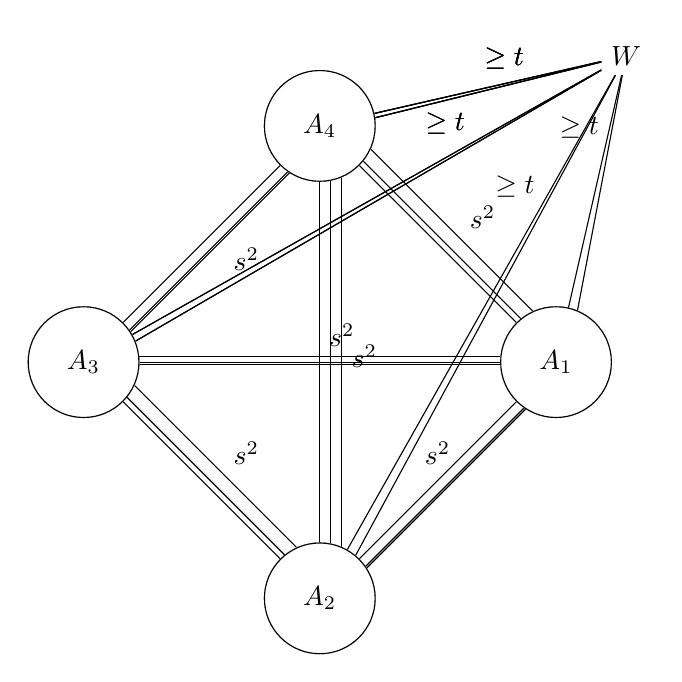
\begin{tikzpicture}
\begin{scope}
% \node[left] at (0,0) {$\circlearrowleft$};

\def\n{4}
\def\radius{.6}
\def\rotation{90}

\def\deg{360/\n}
\pgfmathsetmacro\nminusone{\n-1}

 \pgfmathsetmacro\myangle{-1*.5*\deg+\rotation}

\filldraw[white] (\myangle:5.5cm) circle (10pt);
\draw (\myangle:5.5cm) node[auto](w){$W$};


% do first one
\pgfmathsetmacro\myangley{-1*\deg+\rotation}
\draw (\myangley:3cm) -- (w);
\draw[xshift=4pt,yshift=-1pt] (\myangley:3cm) -- (w) node[near end,auto]{$\geq t$};

% do the rest
\foreach \y in {2,...,\n}
{
\pgfmathsetmacro\yminusone{\y-1}

\foreach \z in {1,...,\yminusone}
{
\pgfmathsetmacro\myangley{-1*\y*\deg+\rotation}
\pgfmathsetmacro\myanglez{-1*\z*\deg+\rotation}
\draw (\myangley:3cm) -- (\myanglez:3cm);
\draw[xshift=4pt,yshift=-1pt] (\myangley:3cm) -- (\myanglez:3cm);
\draw[xshift=8pt,yshift=2pt] (\myangley:3cm) -- (\myanglez:3cm) node[midway,auto]{$s^2$};


\draw (\myangley:3cm) -- (w);
\draw[xshift=4pt,yshift=-1pt] (\myangley:3cm) -- (w) node[near end,auto]{$\geq t$};

}
}
 % do a few by hand
 % \pgfmathsetmacro\myangley{-1*3*120+90}
 % \pgfmathsetmacro\myanglez{-1*5*120+90}
% \draw (\myangley:3cm) -- (\myanglez:2.9cm);



\foreach \x in {1,...,\n}
{
 \pgfmathsetmacro\myangle{-1*\x*\deg+\rotation}

\ifthenelse{\x = \nminusone}{
\filldraw[white] (\myangle:3cm) circle (10pt);
\draw (\myangle:3cm) node[auto]{$\ldots$};
}{
\ifthenelse{\x = \n}{
\filldraw[white] (\myangle:3cm) circle (20pt);
\draw[black] (\myangle:3cm) circle (20pt) node{$A_{k-1}$};
}{
\filldraw[white] (\myangle:3cm) circle (20pt);
\draw[black] (\myangle:3cm) circle (20pt) node{$A_\x$};
}
};

}
\end{scope}
\end{tikzpicture}
\end{center}
\end{figure}
Now, we wish to show $w:= |W|$ is large. First,
\begin{align*}	
\left( \frac{k-2}{k-1}+ \epsilon \right)n(k-1)s &\leq  \sum_{v\in U}\deg(v) \leq \sum_{v\in V(G)} |N(v)\cap U|\\
&\leq \underbrace{w s(k-1)}_{\text{from verticies in }W} + \underbrace{(n-w) (s(k-2)+t)}_{\text{from verticies not in }W}\\
% &= wsn - ws + ns - n(k-2) + nt - ws + w(k-2) - wt\\
% &= wsn - ws + ns - nk + 2n + nt -ws +wk - 2w - wt\\
((k-2) + \epsilon (k-1)) n s &\leq ns (k-2) + nt + w(s-t)
\end{align*}
If we choose $s$ such that $\epsilon (k-1) s -t \geq 1$, then
\[
% &= nsk - 2ns + nt + ws - wt
n \leq n( \epsilon (k-1)s - t) \leq w (s-t) \leq ws.
\]
Then $W\geq \frac{n}{s}$. For each $v\in W$ let $(B_1^v,B_2^v,\dotsc,B_{k-1}^v)$ be the sets of neighbors of $v$ of size $t$ such that $B_i \subset A_i$. There are ${s \choose t}^{k-1}$ choices of these sequences of neighbors, so if $w > \underbrace{s(k-1)}_{\text{vertices in }U}+ (t-1) {s \choose t}^{k-1}$ \marginnote{So $|W\setminus U| \geq |W| - |U| \geq (t-1) {s \choose t}^{k-1}$.} then by pigeonhole principle, there exists $t$  entries in $W\setminus U$ which have the same $t$ neighbors in each of the $A_i$, as desired.\qedhere

\marginnote{The entries in $W\setminus U$ don't need to be independent, because we just need a subgraph, so we can just not include those edges in our subgraph.}


\end{proof}
% section turian_type_problems (end)